
Das folgende Beispiel soll das Visitor-Pattern und die Möglichkeiten, welche sich aus dem Pattern ergeben, besser erklären. In einer Küche gibt es mehrere Sorten Gemüse. Die Variation dieser verschiedenen Sorten ist überschaubar und wird sich nicht mehr ändern. Allerdings ist unklar, welche Operationen auf diese Objekte angewendet werden. Um dieses zu berücksichtigen erstellen wir eine Objektstruktur und verlagern die Operationen auf dieses nicht in den Objekten selbst, sondern außerhalb. Hierfür erstellen wir zunächst ein Interface \texttt{Element} mit der Schnittstelle \texttt{accept(Visitor aVisitor)} und lassen jedes Element unserer Objektstuktur dieses Interface implementieren. Damit verschaffen wir jedem Element die Möglichkeit ein Visitor-Objekt zu erhalten und auf dessen Methoden zuzugreifen.


\begin{listing}[h!]
   \centering
   \javacode{./resources/visitor_element_interface.java}
   \caption{Element Interface}
    \label{visitor_element_interface}
\end{listing}  

Als nächstes erstellen wir das Visitor-Objekt (Listing \ref{visitor_visitor_interface}). Dieses muss für jeden Elementtyp der Objektstruktur eine eigene Methode bereitstellen. Für das Beispiel wurde exemplarisch ein Potato-Element und ein Broccoli-Element erstellt. Für diese beiden Elemente muss das Visitor-Objekt die Methoden definieren, nämlich eine \texttt{visitPotato(Potato)} und \texttt{visitBroccoli(Broccoli)} Methode.


\begin{listing}[h!]
   \centering
   \javacode{./resources/visitor_visitor_interface.java}
   \caption{Visitor Interface}
    \label{visitor_visitor_interface}
\end{listing}  

In Listing \ref{visitor_potato} wird ein konkretes Element vorgestellt. Dieses muss durch das Interface Element die Accept-Methode implementieren und bekommt einen beliebigen Visitor.
In dieser Accept-Methode ruft das Element Potato dann die für ihn gedachte Visitor-Methode, nämlich die \texttt{visitPotato(Potato)} auf und übergibt sich selbst als Potato-Element.

\begin{listing}[h!]
   \centering
   \javacode{./resources/visitor_potato.java}
   \caption{CleanVisitor}
    \label{visitor_potato}
\end{listing}  

Daraufhin kann ein konkreter Visitor, hier der CleanVisitor (siehe Listing \ref{visitor_cleanvisitor}) das übergebene Potato modifizieren. Analog werden jetzt die Visit-Methoden für die anderen Elemente implementiert. Voraussetzung ist allerdings an dieser Stelle, das die jeweiligen Elemente öffentliche Attribute oder Methode bereitstellen, damit diese auch entsprechend bearbeitet werden können.

\begin{listing}[h!]
   \centering
   \javacode{./resources/visitor_cleanvisitor.java}
   \caption{CleanVisitor}
    \label{visitor_cleanvisitor}
\end{listing}  

Abschließend veranschaulicht das Sequenzdiagramm in Abbildung \ref{visitor_sequenzdiagramm}  noch einmal den gesamten Ablauf. Ein beliebiger Client erstellt zunächst die Elemente der Objektstruktur und den Visitor. Dann ruft er bei beiden Elementen mit die Accept-Methode auf und übergibt den Elementen den erstellten konkreten Visitor. Diese rufen ihrerseits die Accept-Methode auf und übergeben sich selbst. Der Visitor ist nun in der Lage die übergebenen Elemente in den dafür vorgesehenen Visit-Methoden zu bearbeiten.


\begin{figure}[htbp]
\centering
%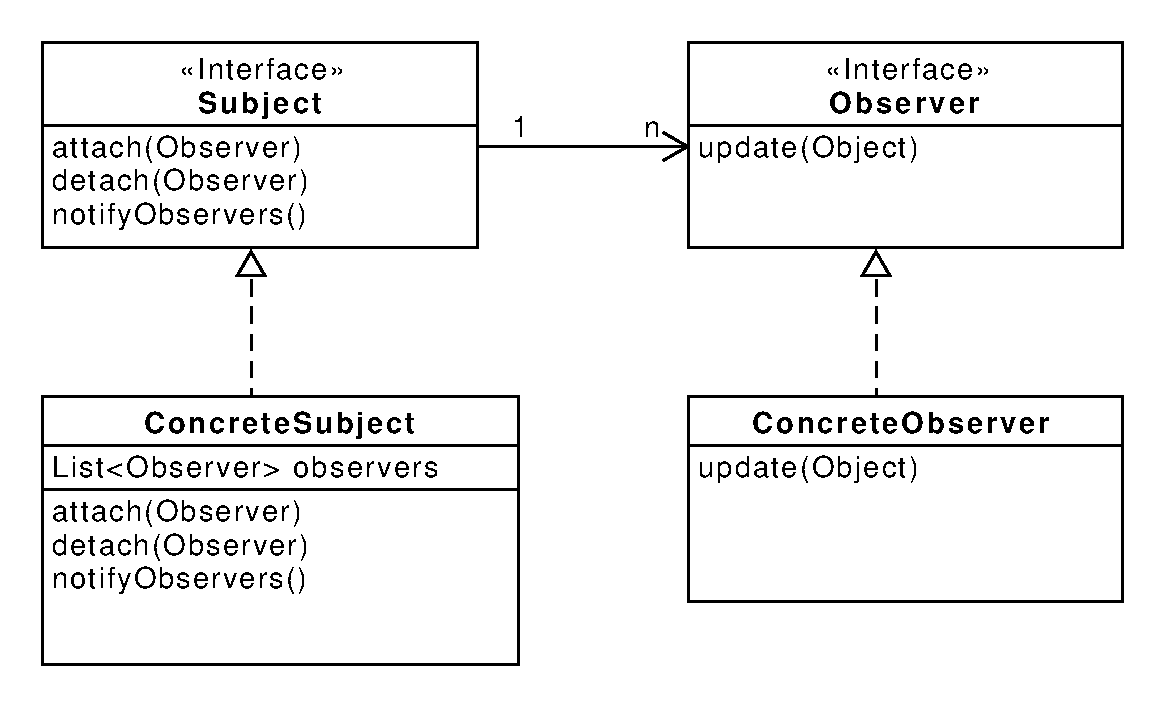
\includegraphics[scale=.5]{./observer/observer}
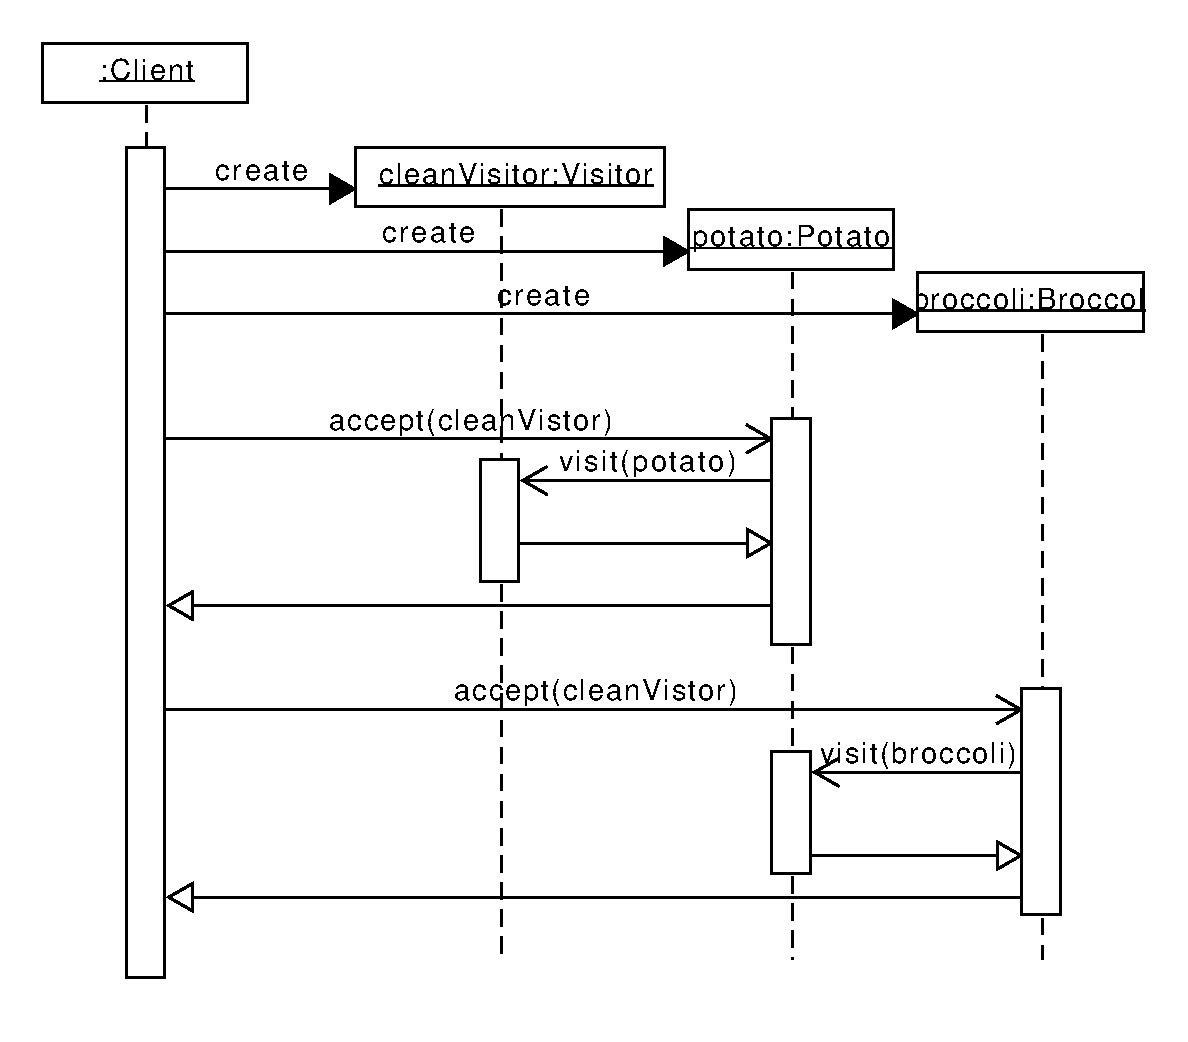
\includegraphics[width=0.5\textwidth]{./paper/visitor/visitor_sequenz}
\caption{Der Ablauf des Visitor-Pattern als Sequenzdiagramm}
\label{visitor_sequenzdiagramm}
\end{figure} 





